\chapter{Paths and connectedness}
\section*{Can every place be reached?}
When a network has no route between some pair of locations, it breaks into separate regions. To reason accurately about routes, distinguish a walk, which may repeat, from a path, which does not repeat vertices.

\begin{definition}
A \emph{walk} is a finite sequence of vertices with consecutive vertices adjacent. A \emph{trail} is a walk that does not repeat edges. A \emph{path} is a walk that does not repeat vertices. A \emph{cycle} is a closed walk of length at least 3 in which no vertex is repeated except that the starting and ending vertices are the same. A graph is \emph{connected} if every pair of vertices is joined by a path; otherwise its maximal connected pieces are its \emph{components}.
\end{definition}

\begin{figure}[htbp]
\centering
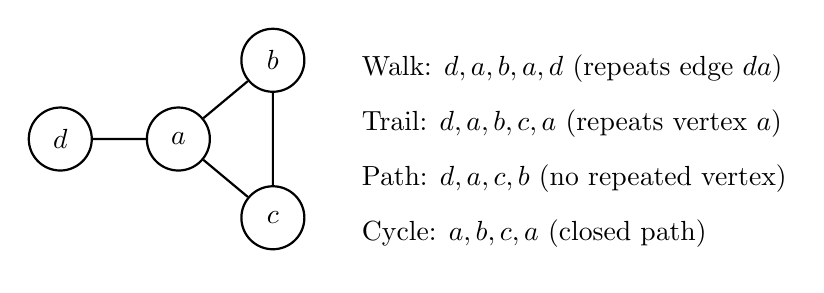
\begin{tikzpicture}[thick,every node/.style={circle,draw,fill=white,minimum size=8mm}]
\node (a) at (0,0) {$a$}; \node (b) at (1.2,1) {$b$};
\node (c) at (1.2,-1) {$c$}; \node (d) at (-1.5,0) {$d$};
\draw (a)--(b)--(c)--(a) (a)--(d);
\node[draw=none,rectangle,anchor=west] at (2.2,0.9) {Walk: $d,a,b,a,d$ (repeats edge $da$)};
\node[draw=none,rectangle,anchor=west] at (2.2,0.2) {Trail: $d,a,b,c,a$ (repeats vertex $a$)};
\node[draw=none,rectangle,anchor=west] at (2.2,-0.5) {Path: $d,a,c,b$ (no repeated vertex)};
\node[draw=none,rectangle,anchor=west] at (2.2,-1.2) {Cycle: $a,b,c,a$ (closed path)};
\end{tikzpicture}
\caption{Walks may repeat edges; trails may repeat vertices; paths repeat neither.}
\end{figure}

\begin{theorem}[\Core{} A walk contains a path]
If there is a $u$--$v$ walk in a graph, then there is a $u$--$v$ path.
\end{theorem}
\begin{proof}
Choose a $u$--$v$ walk of minimum length. If a vertex occurs twice, remove the part of the walk between two of its occurrences. The result is a shorter $u$--$v$ walk, contradicting minimality. Thus no vertex repeats, so the walk is a path.
\end{proof}
This simple fact lets us replace a route that may repeat vertices by one that does not.

\begin{theorem}[\Core{} Bipartite graphs and odd cycles]
A graph is bipartite if and only if it contains no odd cycle.
\end{theorem}
\begin{figure}[htbp]
\centering
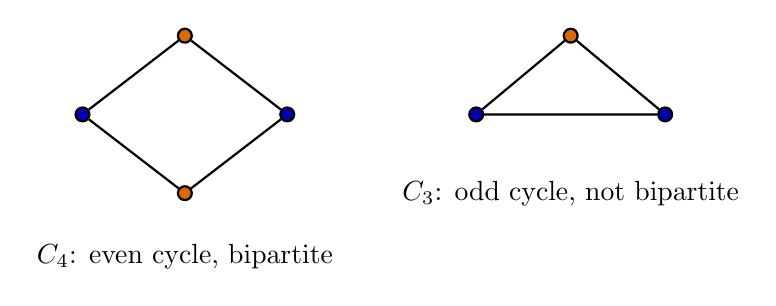
\begin{tikzpicture}[thick,vertex/.style={circle,draw=black,fill=black,inner sep=0pt,minimum size=5pt}]
\node[vertex,fill=blue!70!black] (a) at (0,0) {};
\node[vertex,fill=orange!85!black] (b) at (1.3,1) {};
\node[vertex,fill=blue!70!black] (c) at (2.6,0) {};
\node[vertex,fill=orange!85!black] (d) at (1.3,-1) {};
\draw (a)--(b)--(c)--(d)--(a);
\node[draw=none,rectangle,fill=white] at (1.3,-1.8) {$C_4$: even cycle, bipartite};
\node[vertex,fill=blue!70!black] (p) at (5,0) {};
\node[vertex,fill=orange!85!black] (q) at (6.2,1) {};
\node[vertex,fill=blue!70!black] (r) at (7.4,0) {};
\draw (p)--(q)--(r)--(p);
\node[draw=none,rectangle,fill=white] at (6.2,-1) {$C_3$: odd cycle, not bipartite};
\end{tikzpicture}
\caption{Alternating two classes succeeds around an even cycle but fails around an odd one.}
\end{figure}
\begin{proof}
If a graph is bipartite, a walk alternates between the two vertex classes at each step. Returning to the starting class therefore takes an even number of steps, so every cycle has even length.

Conversely, suppose the graph has no odd cycle. Work within one component and choose a starting vertex $r$. Put each vertex in one of two classes according to whether its shortest-path distance from $r$ is even or odd. If an edge joined two vertices at the same parity, shortest paths from $r$ to those endpoints together with the edge would contain an odd closed walk. Every odd closed walk contains an odd cycle: if any vertex appears at two occurrences beyond the required equality of the first and last vertices, split the walk at those occurrences. The two shorter closed walks have lengths summing to the original odd length, so one is odd. Keep that shorter odd closed walk and repeat; because the lengths decrease, this process ends with an odd cycle. This contradicts the assumption. So each edge joins opposite classes. Repeat for each component.
\end{proof}

\section*{Breadth-first search: exploring by layers}
Breadth-first search (BFS) explores a graph from a chosen starting vertex in layers: first the start, then vertices one edge away, then vertices two edges away, and so on. In an unweighted graph, the first path found to a vertex uses the fewest edges.

To find a path from a source $s$ to a target $t$:
\begin{enumerate}
\item Put $s$ in a first-in, first-out queue, mark it as discovered, and record that it has no predecessor.
\item Remove the vertex $u$ at the front of the queue and inspect each of its neighbours.
\item For every neighbour $v$ not yet discovered, mark $v$ as discovered, record $u$ as its predecessor, and add $v$ to the back of the queue.
\item Continue until $t$ is discovered or the queue is empty. If $t$ is discovered, follow the predecessor records back to $s$ to recover a shortest path in number of edges.
\end{enumerate}

For the Town Hall journey, BFS would find a route using the fewest road segments if each road segment counts as one edge. It does not necessarily find the fastest route when segments have different travel times: a route with more quick segments can take less time than one with fewer slow segments. The Dijkstra section later in the book explains how to handle non-negative travel-time weights. Depth-first search (DFS), by contrast, follows one branch as far as possible before backtracking. BFS and DFS can both be implemented with a queue or stack and a set of discovered vertices.

\section*{Exercises}
\begin{enumerate}
\item In a square with one diagonal, list a walk of length 4 that is not a trail, and a trail that is not a path.
\item Is a 7-cycle bipartite? Justify your answer. What about a 10-cycle?
\item Draw a disconnected graph with exactly three components and list their sizes.
\item \Coding{} Starting at a chosen vertex, perform BFS on a graph of your own design and record the order vertices are first visited. Compare with DFS.
\end{enumerate}
